\documentclass[11pt]{amsbook}

\usepackage{../HBSuerDemir}

\begin{document}
	\hPage{341}
	determinantal equation is \\\\
	$\begin{vmatrix}
		x&  y&  l \\
		\sum{x_i}& \sum{y_i}&  n \\
		\sum{x_i^2}& \sum{x_iy_i}& \sum{x_i}
	\end{vmatrix}$ $ = 0 $ or  
	$\begin{vmatrix}
	x&  y&  l \\
	\overline{x}& \overline{y}&  l \\
	\sum{x_i^2}& \sum{x_iy_i}& \sum{x_i}
	\end{vmatrix}$ $ = 0 $  \\
	
	 The second row in the last equation show that the line of best fit passes through the point $P (\overline{x}, \overline{y}) $. \\
	 
	 Observe that the first equation in $ (l) $ for parameters can be obtained practically from $ y_i = Ax_i + B $ by summation; and the second by summation after multiplying by $ x_i $. \\
	 
	 \underline{Example}. Given the data \\
	 \begin{figure}[htbp]
	 	\centering
	 	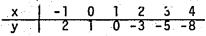
\includegraphics[width=0.45\textwidth]{images/b2p2-341-fig1.png}
	 \end{figure} \\ 
	find the equation of the line of best fit. \\
	\hspace{5pt} \underline{Solution}. \\
	
	\begin{minipage}{0.3\textwidth}
		\raggedright
		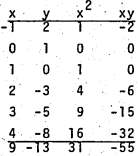
\includegraphics[width=\linewidth]{images/b2p2-341-fig2.png} 
	\end{minipage}% 
    \hfill%
	\begin{minipage}{0.6\textwidth}\raggedright
			\[ \Longrightarrow 9A + 6B = -13 \]\\
		\[31A + 9B = -55 \]\\
		\[ \Longrightarrow A = -\dfrac{213}{105}, B = \dfrac{92}{105} \] \\
		\[ \Longleftrightarrow y= -\dfrac{213}{105}x + \dfrac{92}{105} \] \\
		\[ = -2,028x + 0,876\]
	\end{minipage} \\\\
		Where there are more than one variable, say two variables, in the case of linear approximation the general linear equation is \\
		
		 $ z= Ax+By+C $ , \\
		 
		and by the $MLS$ one may obtain the following equations for parameters:

		
	
	 
	 
	
\end{document}
	 
 